\subsubsection{Calibration}
Calibration is the operation of setting the energy each channel corresponds to.

\begin{figure}[H]
    \centering
    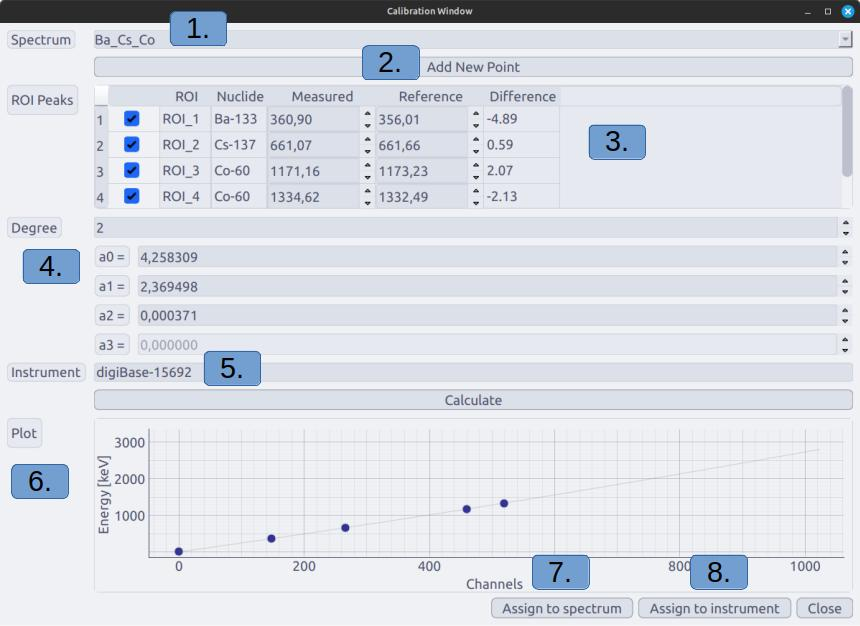
\includegraphics[width = .7\linewidth]{images/interface/gtools_calibration.jpg}
    \caption{Calibration window of a spectrum with 4 ROIs and assigned nuclides.}
    \label{fig:gtools_calibration}
    \begin{flushleft}
        \begin{enumerate}
            \item Which spectrum should be used for the calibration. For each calibration, data from only one spectrum is allowed.
            \item Add a calibration point, that is not associated with a ROI. Measured and Reference energies must be set manually.
            \item Current calibration points detected and their corresponding information. When unchecking a row it will be ignored in the calculation.
            \item Polynomial degree of the calibration function and the current coefficients. Coefficients can be changed manually but will be updated by pressing \texttt{Calculate}.
            \item The instrument used for acquiring the spectrum. This is fixed and can not be changed here, instead edit the spectrum before starting the calibration, see section \ref{}.
            \item Plot showing the energy as a function of channels based on the latest calculated coefficients.
            \item Assign the coefficients to the \textit{Unique Instrument} shown in (5.).
            \item Assign the new calibration coefficients and recalculate the x-axis for the spectrum selected in (1.), updating the view in the Spectrum-tab. Note, this will not change the calibration of an already started spectrogram.
        \end{enumerate}
    \end{flushleft}
\end{figure}